% Default mode is landscape, which is what we want, however dvips and
% a0poster do not quite do the right thing, so we end up with text in
% landscape style (wide and short) down a portrait page (narrow and
% long). Printing this onto the a0 printer chops the right hand edge.
% However, 'psnup' can save the day, reorienting the text so that the
% poster prints lengthways down an a0 portrait bounding box.
%
% 'psnup -w85cm -h119cm -f poster_from_dvips.ps poster_in_landscape.ps'

\documentclass[a0]{a0poster}
% You might find the 'draft' option to a0 poster useful if you have
% lots of graphics, because they can take some time to process and
% display. (\documentclass[a0,draft]{a0poster})

\pagestyle{empty}
\renewcommand{\d}{\mathrm{d}}
\newcommand{\sgn}[1]{\mathop{\mathrm{sgn}}#1}
\newcommand{\bu}{\mathbf{u}}
\newcommand{\bx}{\mathbf{x}}
\newcommand{\br}{\mathbf{r}}
\newcommand{\ds}{\mathrm{d}s}
\newcommand{\ie}{\textit{i.e.}}
\setcounter{secnumdepth}{0}
\newcommand{\comment}[1]{}

% The textpos package is necessary to position textblocks at arbitary 
% places on the page.
\usepackage[absolute]{textpos}

% Graphics to include graphics. Times is nice on posters, but you
% might want to switch it off and go for CMR fonts.
\usepackage{graphics}
\usepackage{wrapfig,helvet}
\usepackage{amsmath}
%for math
\usepackage{amsfonts}
\usepackage{amssymb}
\usepackage{mathrsfs}


% These colours are tried and tested for titles and headers. Don't
% over use color!
\usepackage{color}
\definecolor{DarkBlue}{rgb}{0.1,0.1,0.5}
\definecolor{Red}{rgb}{0.9,0.0,0.1}
\definecolor{headingcol}{rgb}{0.5,0.7,1}
%\definecolor{boxcol}{rgb}{0.3,0.8,0.1}

% see documentation for a0poster class for the size options here
\let\Textsize\normalsize
\def\Head#1{\noindent\hbox to \hsize{\hfil{\LARGE\color{DarkBlue}\sf #1}}\bigskip}
\def\LHead#1{\noindent{\LARGE\color{DarkBlue}\sf #1}\bigskip}
\def\Subhead#1{\noindent{\large\color{DarkBlue}\sf #1}\bigskip}
\def\Title#1{\noindent{\VeryHuge\color{Red}\bf\sf #1}}

\usepackage{titlesec}
\titleformat{\section}{\normalfont\Huge\bfseries\color{red}}{\thesection.}{1em}{}

\TPGrid[40mm,40mm]{23}{12}  % 3 cols of width 7 plus 2 gaps width 1

\parindent=0pt
\parskip=0.5\baselineskip

\makeatletter							%Needed to include code in main file
\renewcommand\@maketitle{%
\null									%Sets position marker
{
\color{headingcol}\sffamily\VERYHuge		%Set title font and colour
\@title \par}%
\vskip 0.6em%
{
\color{white}\sffamily\LARGE				%Set author font and colour
\lineskip .5em%
\begin{tabular}[t]{l}%
\@author
\end{tabular}\par}%
\vskip 1cm
\par
}
\makeatother

\title{Cauchy-Crofton Formula}

\author{Aadil, Caroline, Chris, Paul}

\begin{document}
%----------------------------------------------------------------------%
%           Title bar: across all 21 columns                           %
%----------------------------------------------------------------------%
\begin{textblock}{23}(0,0)
\vspace*{-115mm}\hspace*{-42mm}%

\includegraphics{ucl_bar_black.eps}
\begin{minipage}{1191mm}		%Minipage for title contents
\vspace{-14cm}
\maketitle
\end{minipage}
\end{textblock}

%%%%%%%%%%%%%%%%%% Will need to shift all other content down a bit %%%%%

%----------------------------------------------------------------------%
%           First column.                                              %
%----------------------------------------------------------------------%
\begin{textblock}{7}(0,1.4)
\Head{Theorem Statement}
$$ \iint_S \,d\rho\,d\theta = 2* l$$


\section{Explanations}


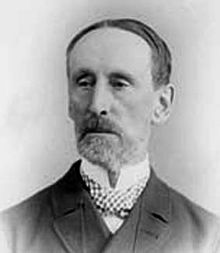
\includegraphics{Morgan_Crofton.jpg}

\end{textblock}

\begin{textblock}{7}(0,8.70)

\end{textblock}

%----------------------------------------------------------------------%
%           Second column.                                             %
%----------------------------------------------------------------------%
\begin{textblock}{7}(8,2.4)
test
\end{textblock}

\begin{textblock}{7}(8,5.25)
test

\begin{center}
\rotatebox{-90}{\scalebox{2.22}{\includegraphics{fig2.eps}}}
\end{center}
\begin{center}
\rotatebox{-90}{\scalebox{22.2}{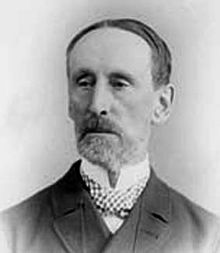
\includegraphics{Morgan_Crofton.jpg}}}
\end{center}

\end{textblock}

%----------------------------------------------------------------------%
%           Third column.                                                     %
%----------------------------------------------------------------------%
\begin{textblock}{7}(16,1)

\section{Applications}
\subsection{Length of a circle}
Take a circle $C$ of radius $r$.
We need to measure the set of lines that crosses the circle, counted with multiplicity:


\scalebox{0.3}{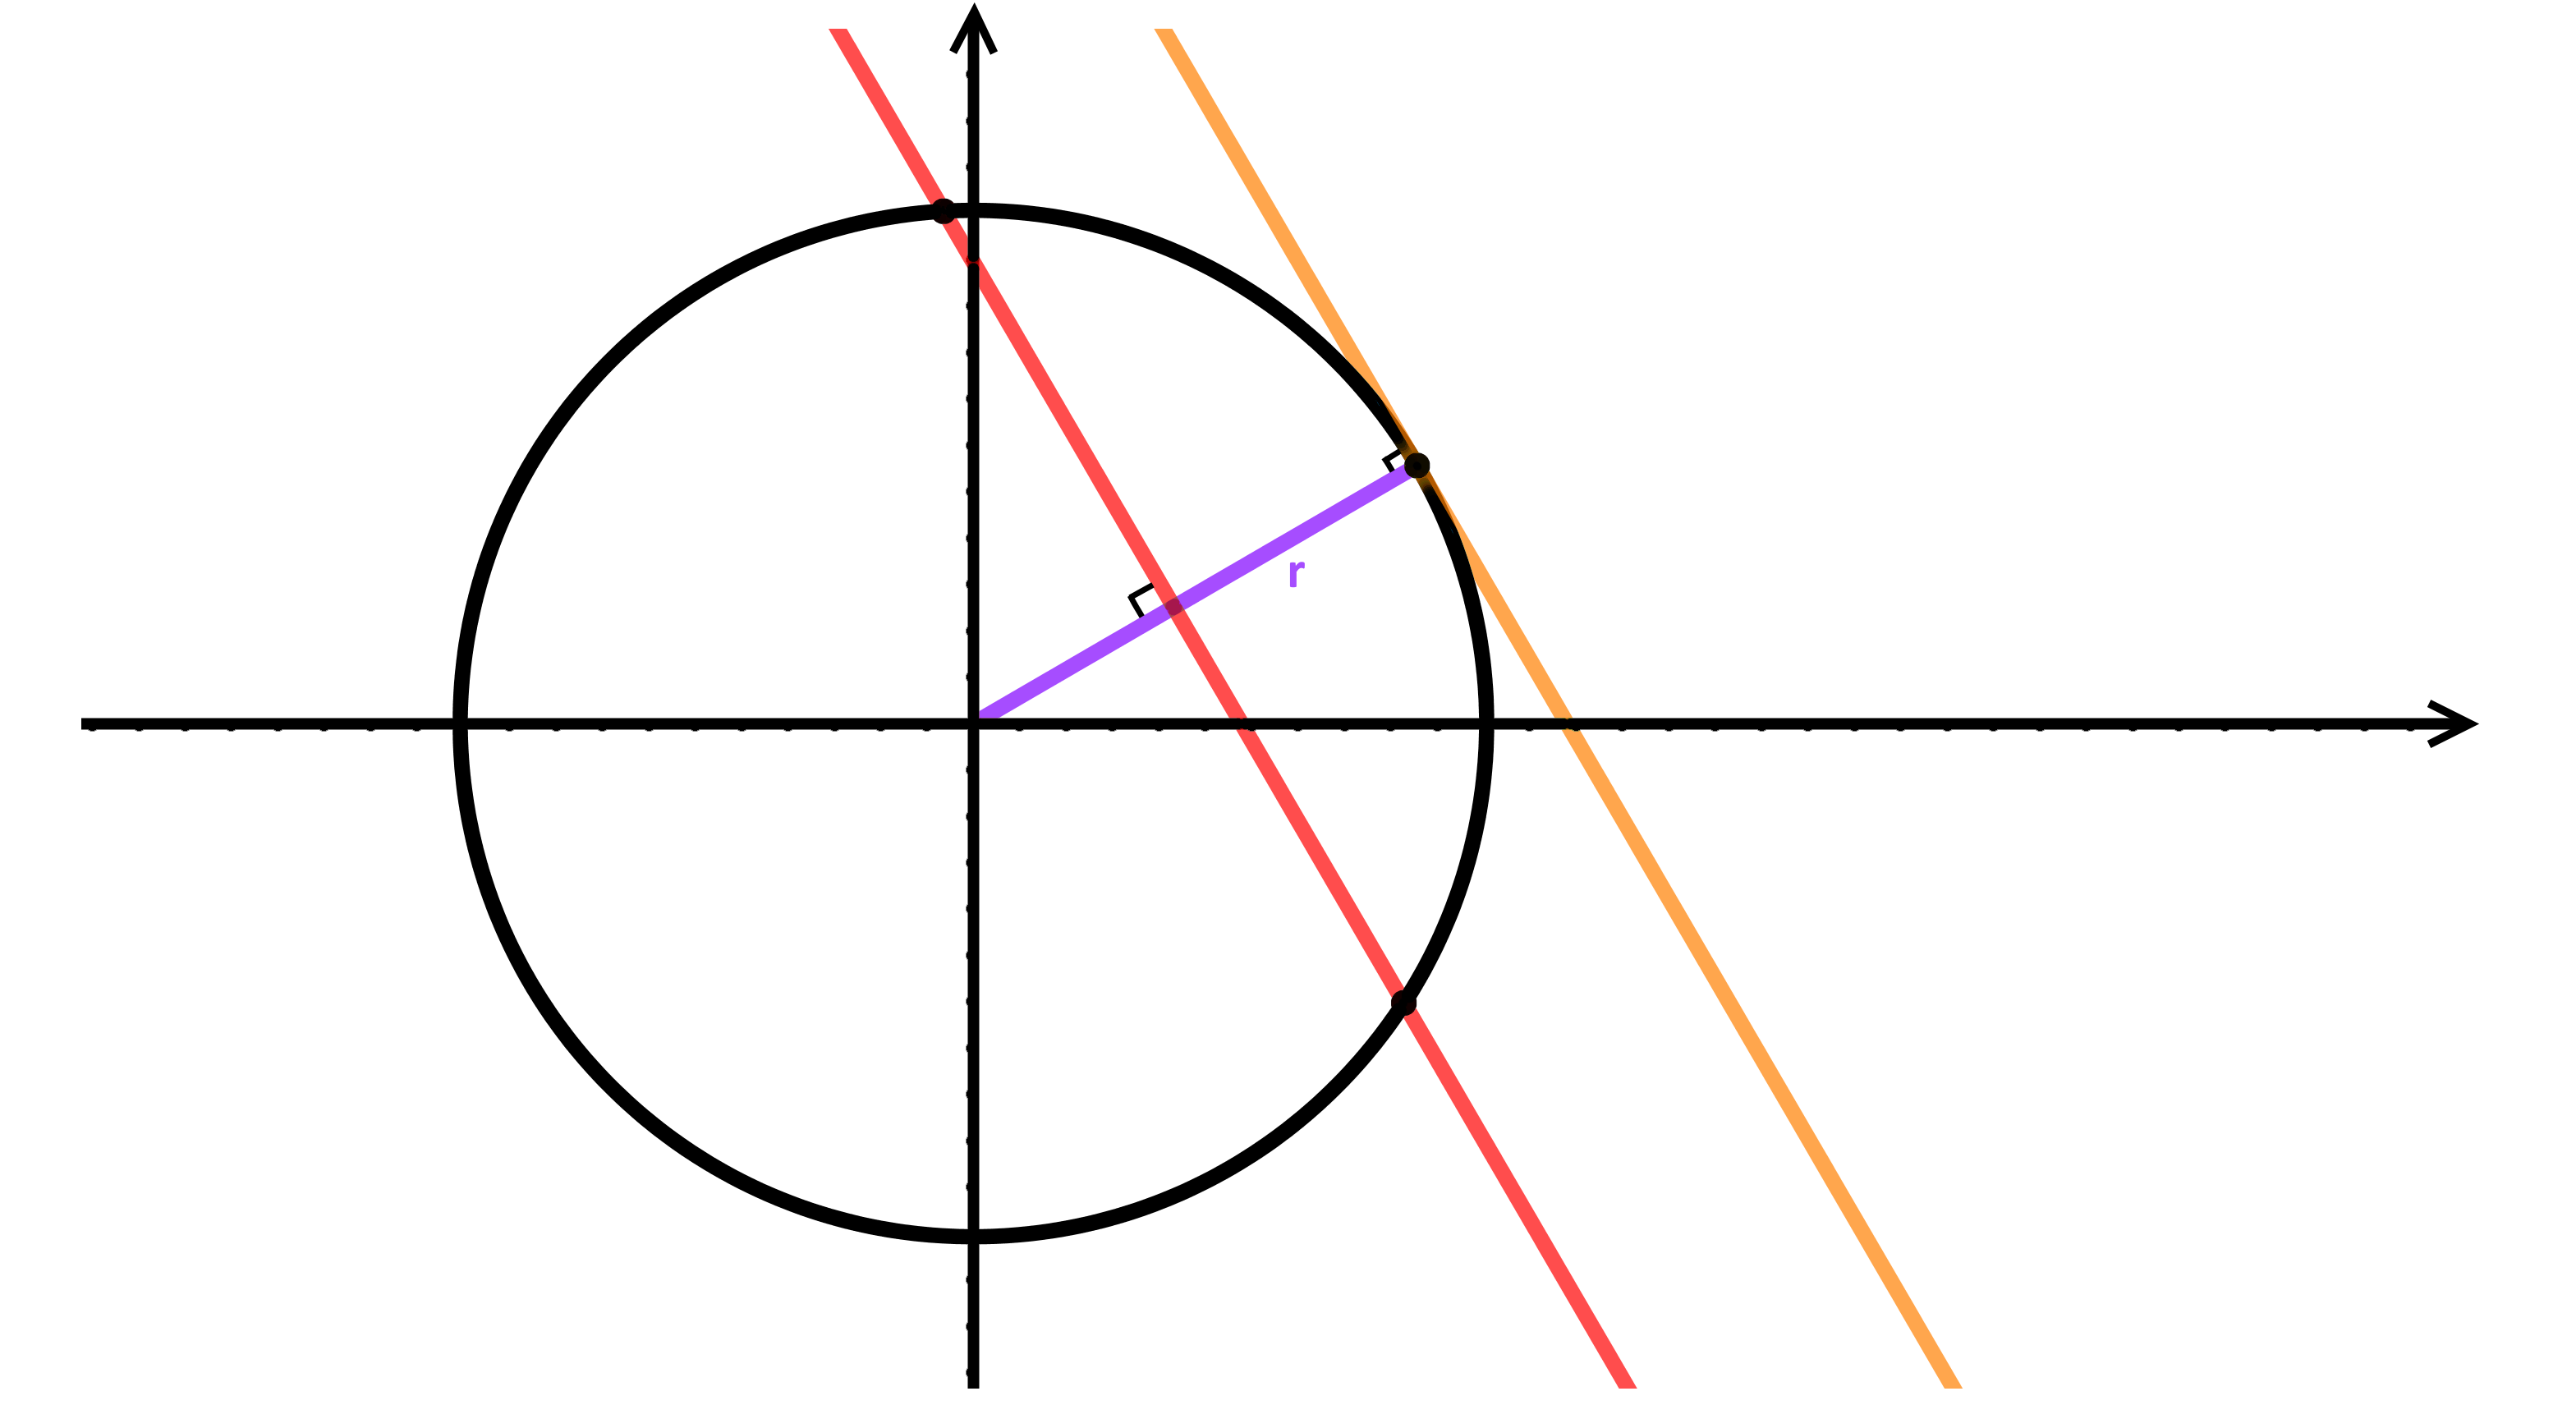
\includegraphics{figureCircleExample.png}}
%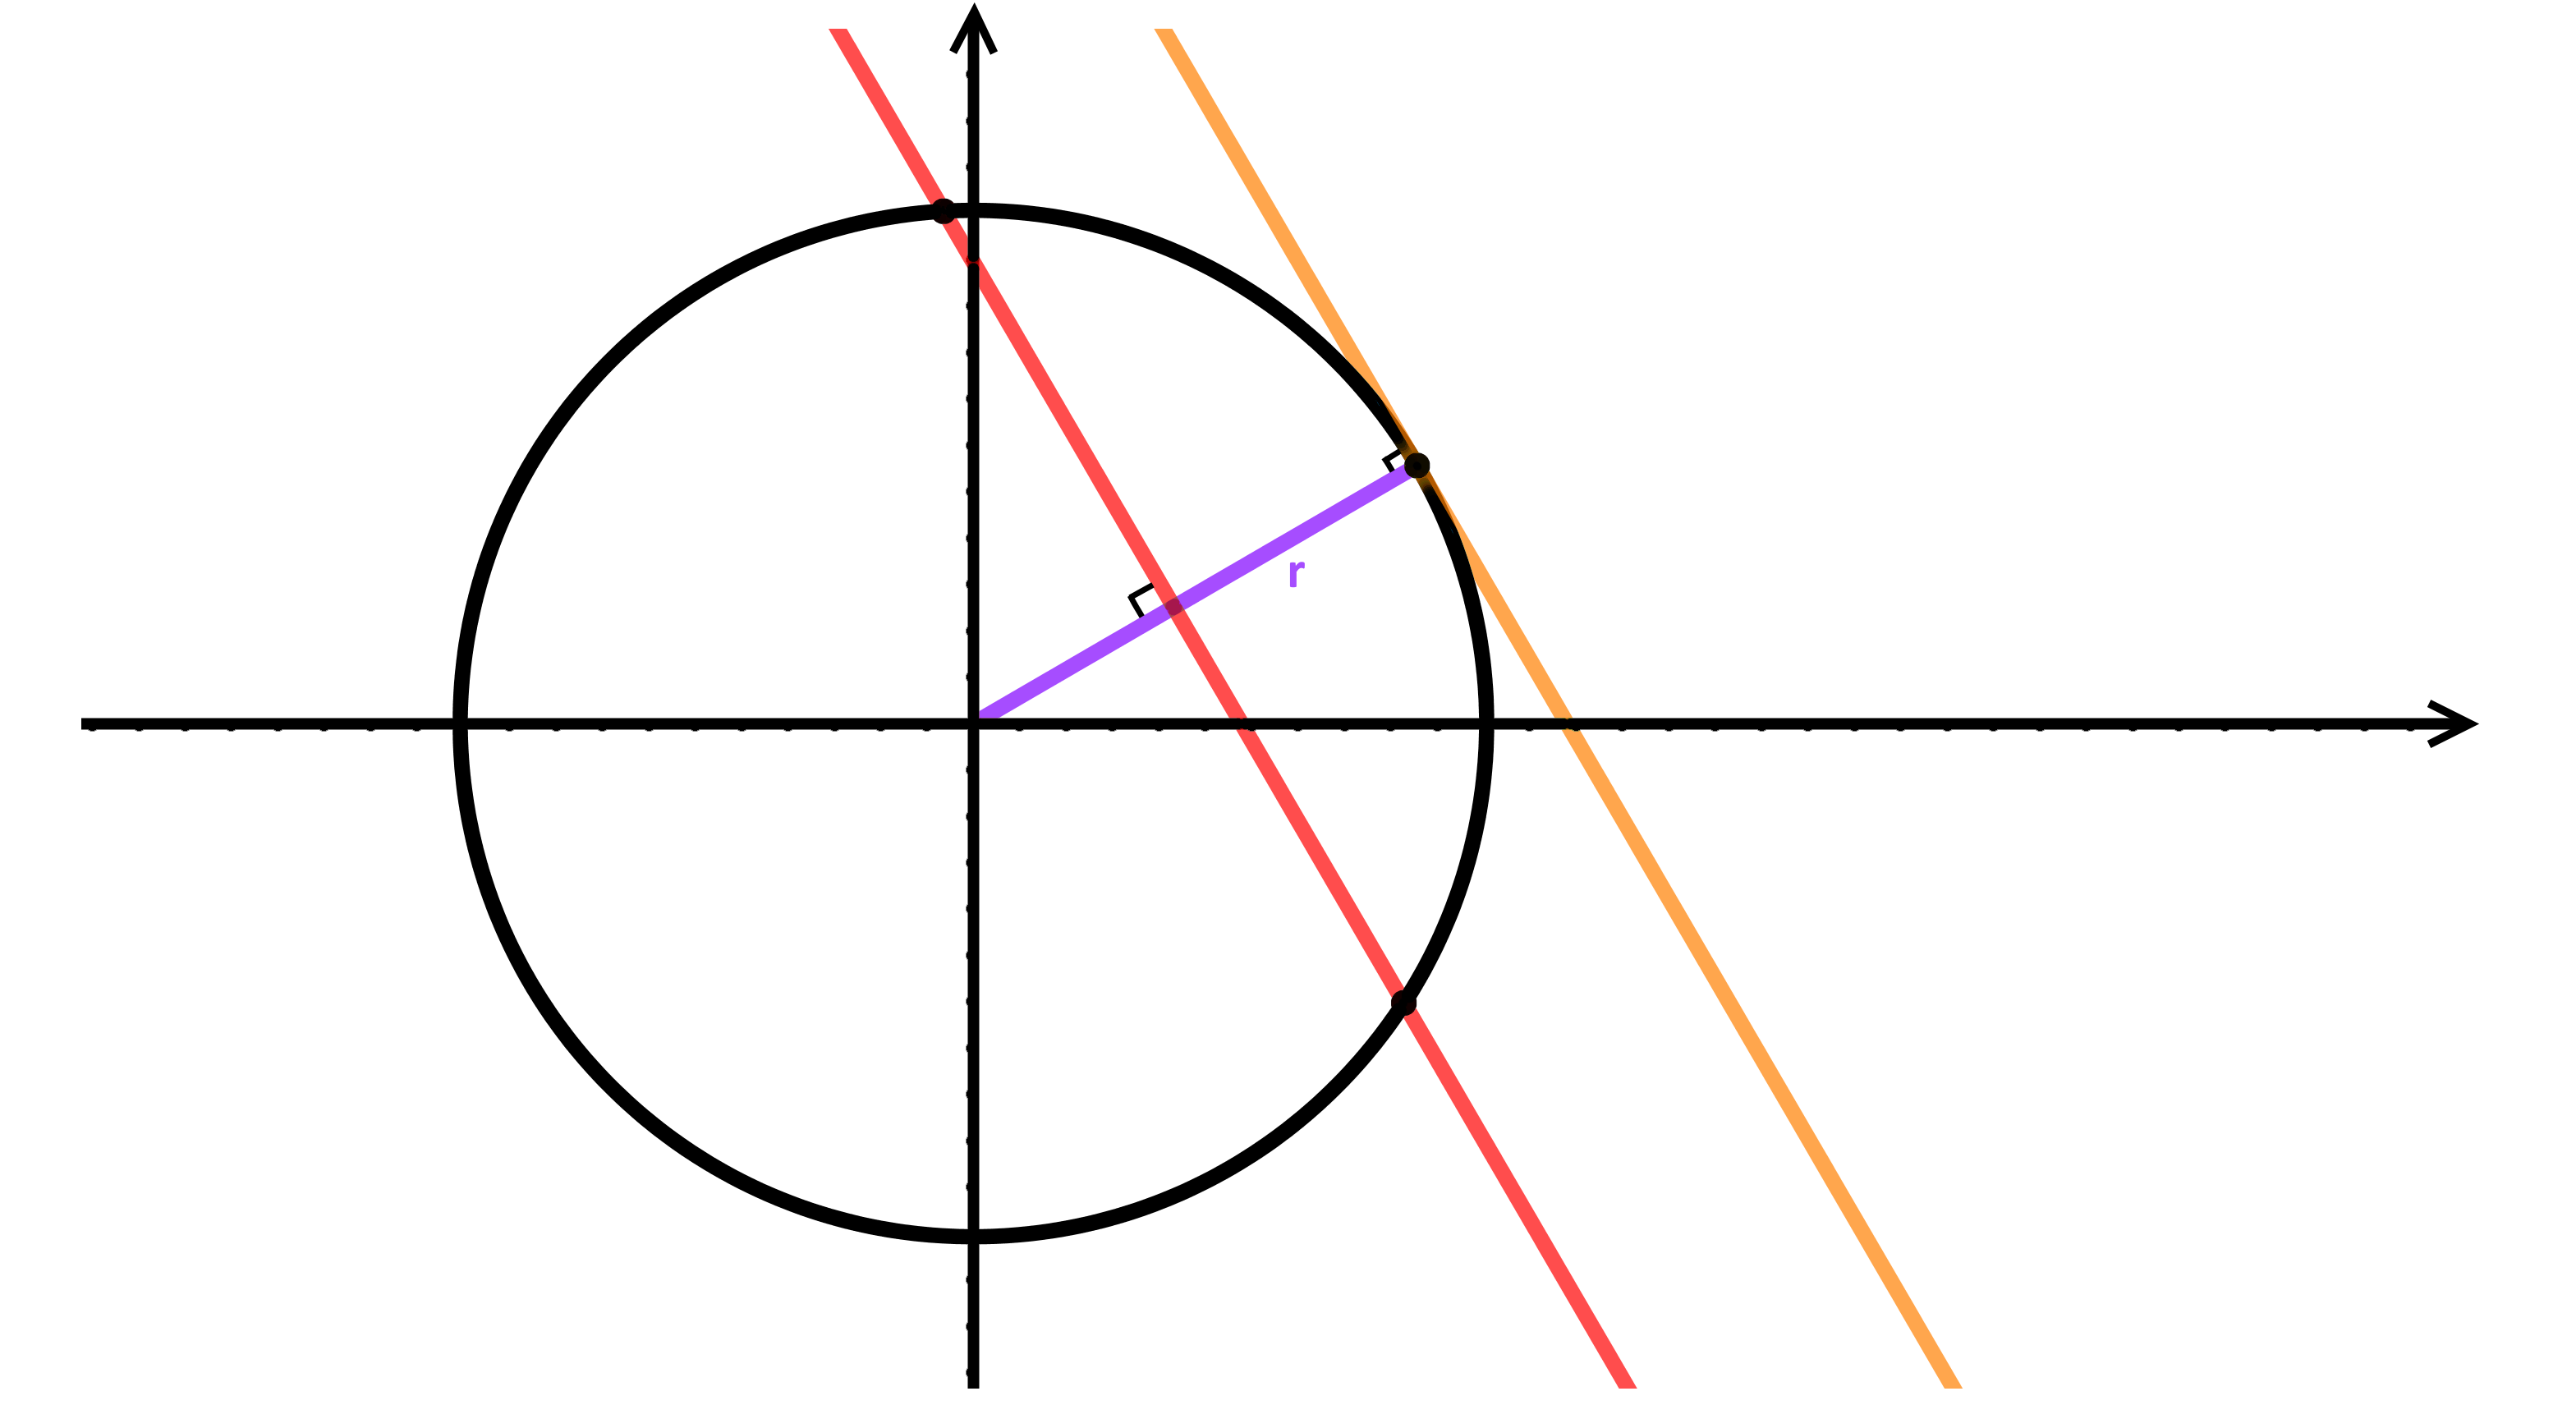
\includegraphics[width=350pt]{figureCircleExample.png}
Here, we get that $\forall 0 \leq \theta \leq 2\pi$, the line represented by $(\rho, \theta)$ is crossing the circle once if $\rho = r$, twice if $\rho < r$ and none if $\rho > r$.
So let $f:\mathbb{R} \to \mathbb{R}$ be such that:
$$f(x) = \left\{
\begin{array}{r c l}
2 \quad if \ x < r\\
1 \quad if \ x = r\\
0 \quad if \ x > r
\end{array}
\right.$$
Thus, the measure of the set of lines crossing $C$ counted with multiplicity is:
\begin{align}
m(C) =& \int_0^{2\pi}\int_0^{+\infty} f(x) dx\,d\theta \\
=& \int_0^{2\pi}\int_0^{r} 2 \ dx\,d\theta \\
=& \int_0^{2\pi} 2 r \ d\theta \\
=& \ 4 \pi r = 2* 2\pi r
\end{align}
And we already know that this is twice the length of the circle of radius $r$.
Therefore, we checked the formula for circles.




\end{textblock}

%----------------------------------------------------------------------%
%            Construction lines                                        %

%\begin{textblock}{23}(0,2)\rule{\textwidth}{0.1mm}\end{textblock}
% Shows where the bottom of the header bar should fall.

%\begin{textblock}{23}(0,2.4)\rule{\textwidth}{0.1mm}\end{textblock}
% Shows where the top of each column should start.

%\begin{textblock}{23}(0,12)\rule{\textwidth}{0.1mm}\end{textblock}
% Shows where the bottom of the lowest block in each column should end

%\begin{textblock}{1.5}(6,4.12)\rule{\textwidth}{0.1mm}\end{textblock}
%\begin{textblock}{1.5}(6,4.52)\rule{\textwidth}{0.1mm}\end{textblock}
% Used to find the base of the first block and thus the top of the second.

%\begin{textblock}{1.5}(14,4.85)\rule{\textwidth}{0.1mm}\end{textblock}
%\begin{textblock}{1.5}(14,5.25)\rule{\textwidth}{0.1mm}\end{textblock}
% Same purpose but in the second column.

%\begin{textblock}{1.5}(15,6.05)\rule{\textwidth}{0.1mm}\end{textblock}
%\begin{textblock}{1.5}(15,6.45)\rule{\textwidth}{0.1mm}\end{textblock}
% Same purpose but in the third column.

\end{document}
